% Appendix A

\chapter{Supplementary figures} % Main appendix title
\chaptermark{Supplementary figures}
\label{AppendixA} % For referencing this appendix elsewhere, use \ref{AppendixA}

%\lhead{Appendix C. \emph{Statistical Tests}} % This is for the header on each page - perhaps a shortened title

\begin{figure}[h!]
\centering
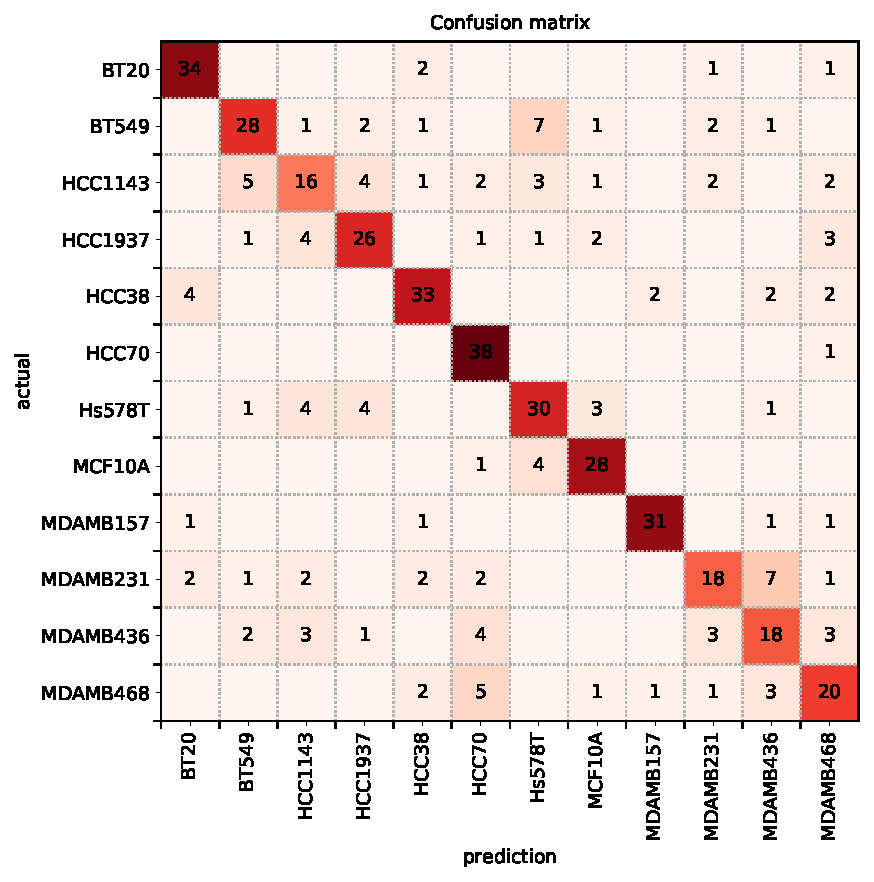
\includegraphics[width=0.8\textwidth]{img/confusion_matrix.pdf}
\caption{Confusion matrix for a random forest classifier classifying cells from $12$ TNBC cell lines.}
\label{fig:confusion_matrix}
\end{figure}

\begin{sidewaysfigure}
\centering
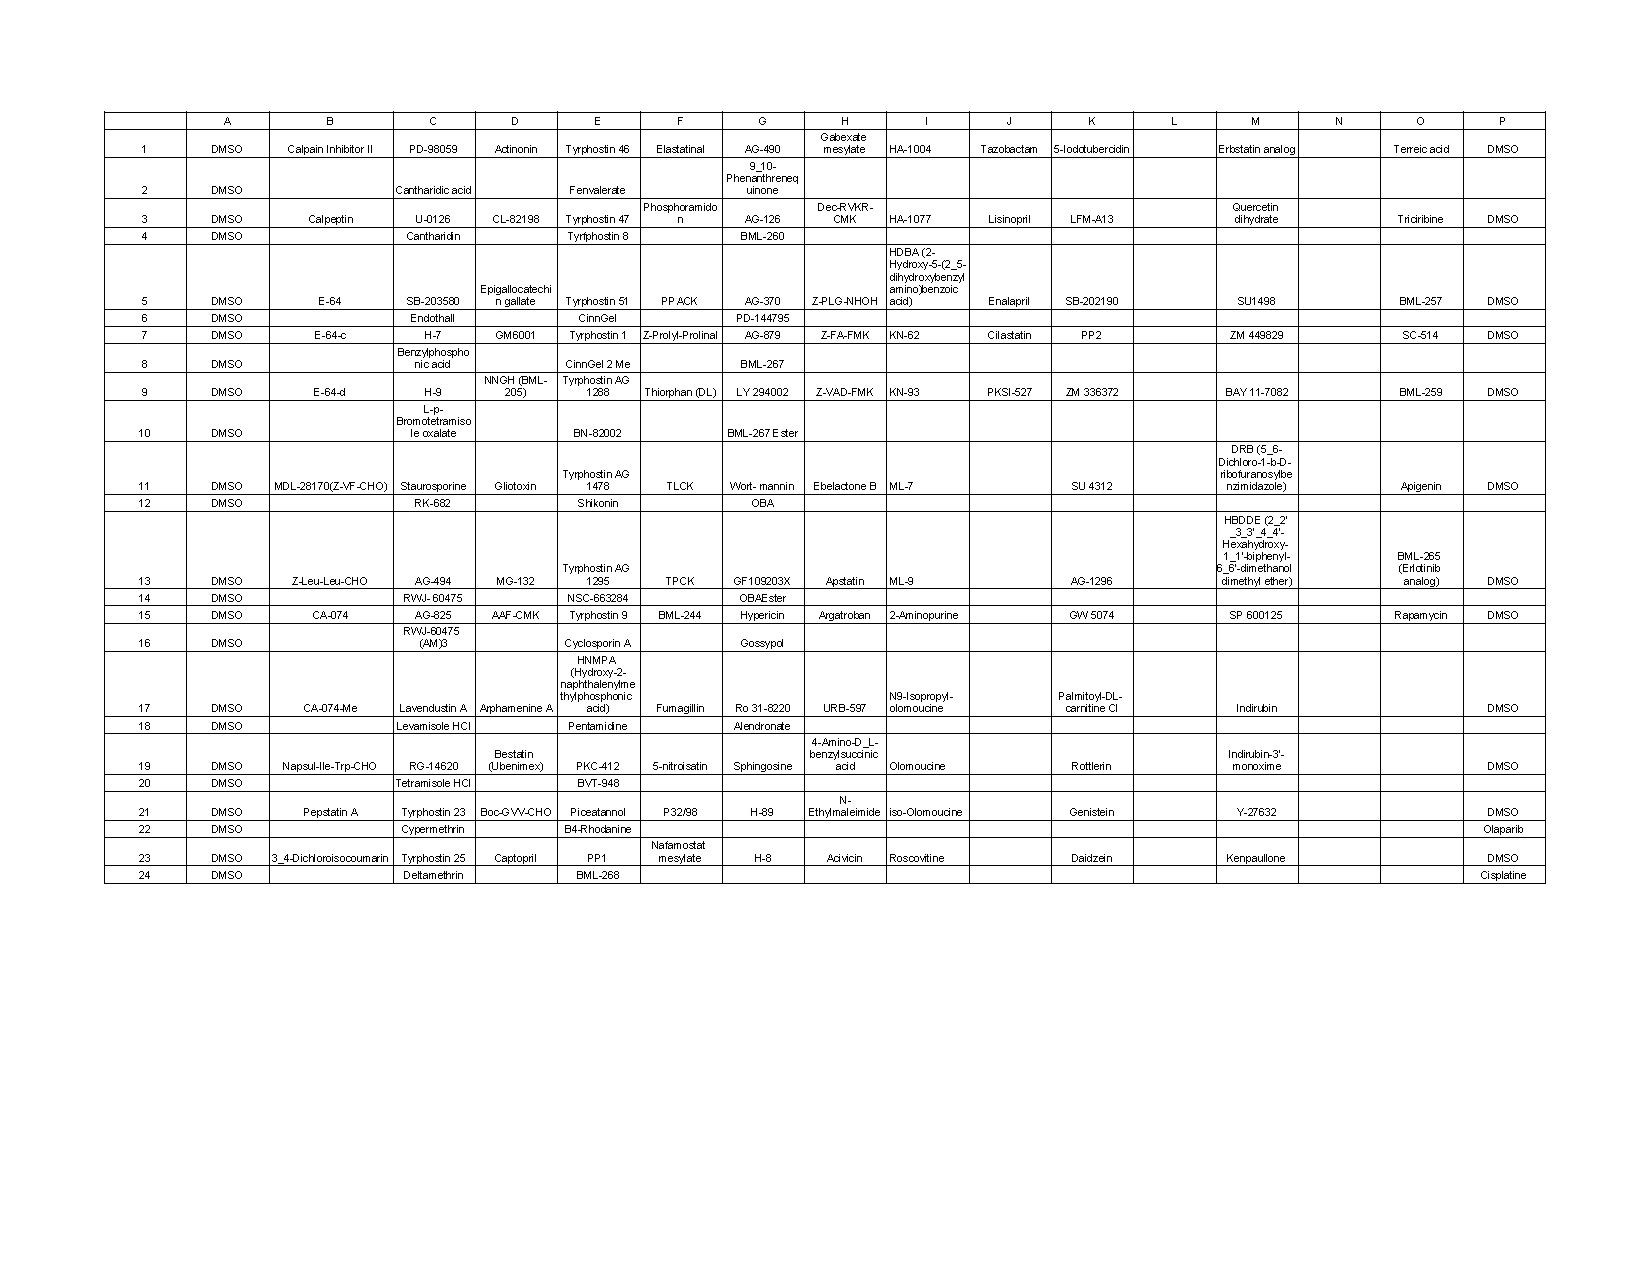
\includegraphics[width=\textwidth]{img/plate_map.pdf}
\caption{Plate map of perturbations used for drug screen. Empty cells indicate empty wells. DMSO denotes negative controls.}
\label{fig:plate_map_sideways}
\end{sidewaysfigure}

\begin{figure}[!ht]
     \subfloat[Endothall takes effect in cell line MDA231 only.\label{subfig-1:dummy}]{%
       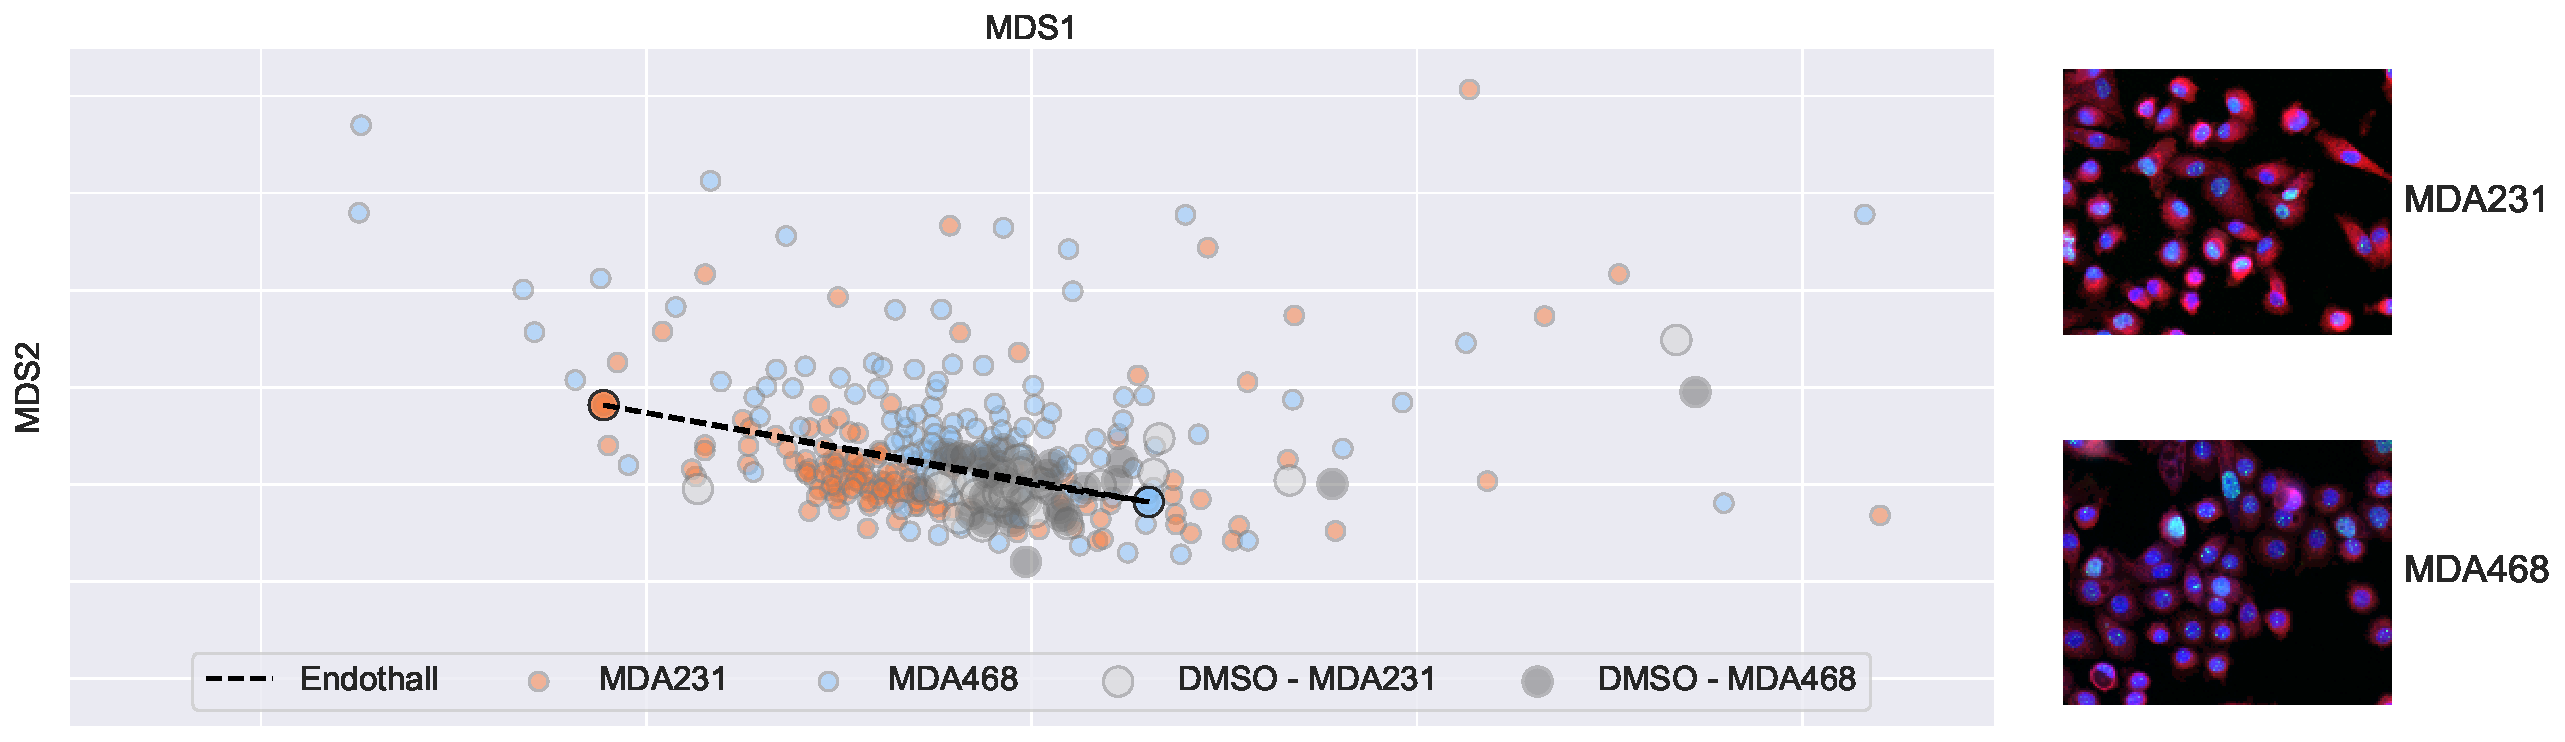
\includegraphics[width=\textwidth]{img/endothall.pdf}
     }
     \hfill
     \subfloat[CL-82198 takes effect in cell line MDA468 only.\label{subfig-2:dummy}]{%
       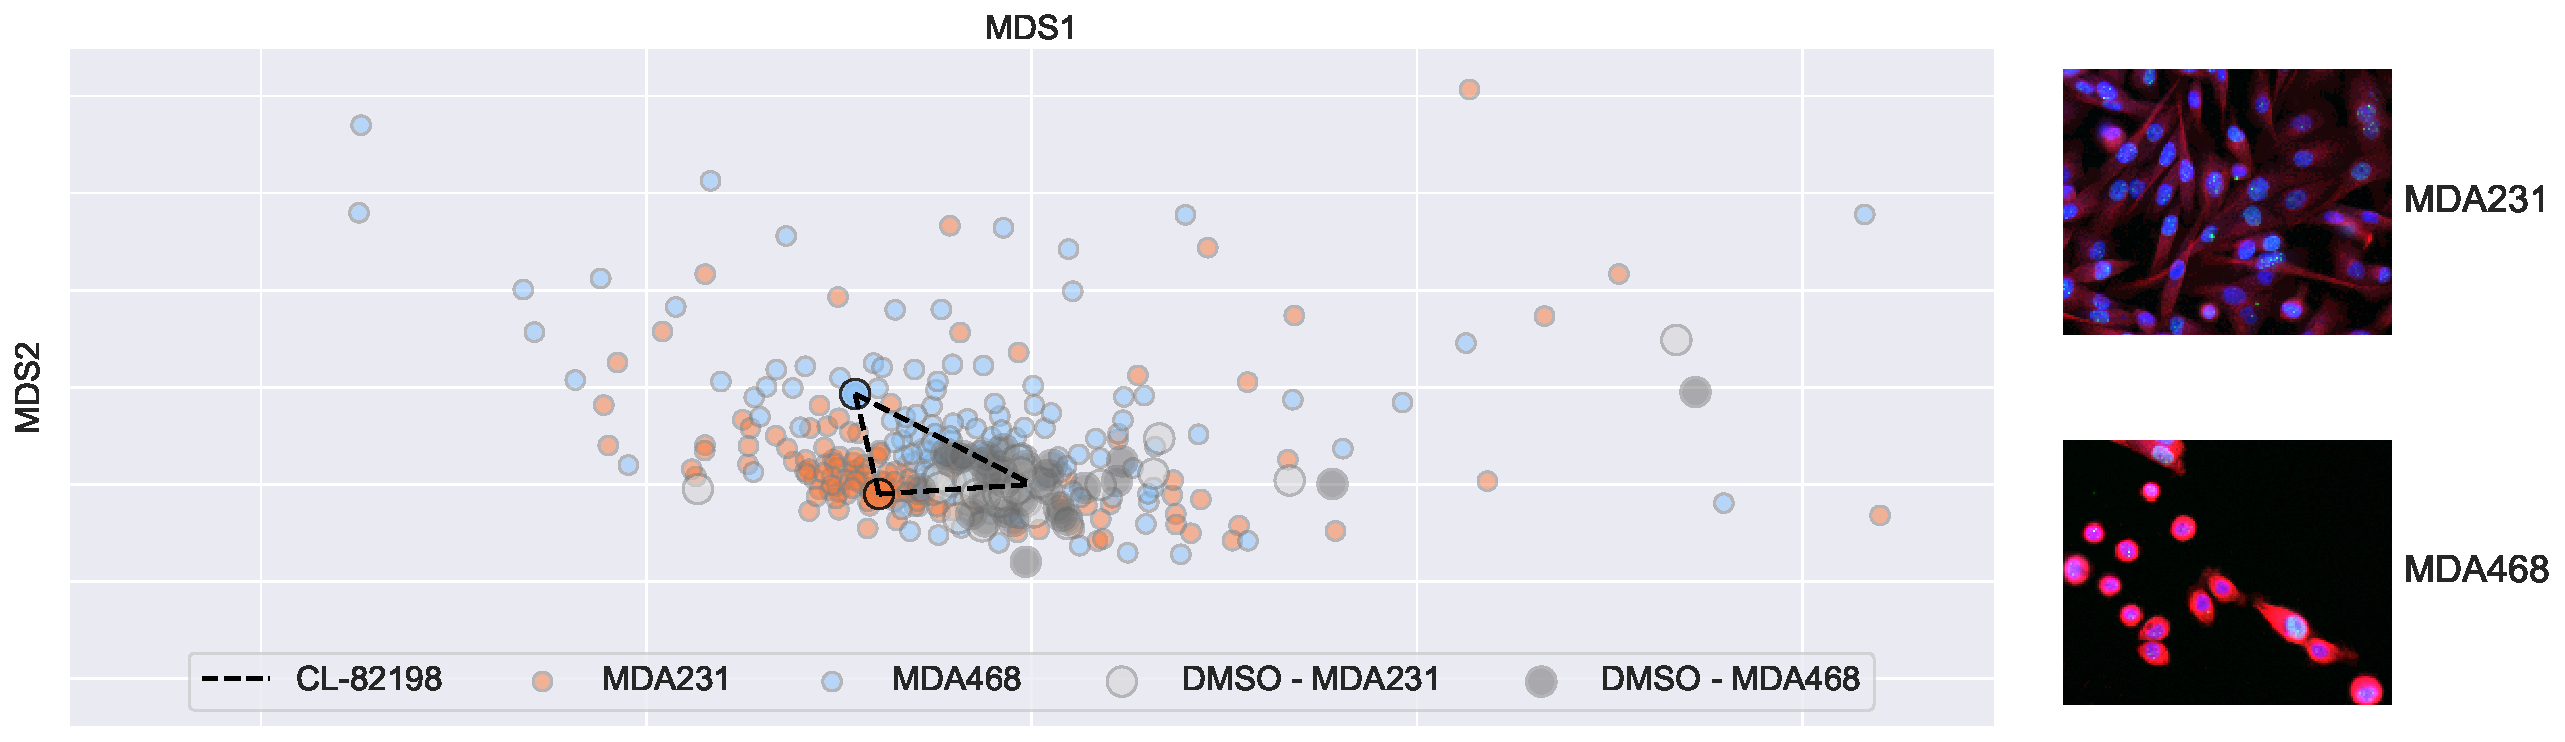
\includegraphics[width=\textwidth]{img/cl-82198.pdf}
     }
     \hfill
     \subfloat[Cyclosporin A takes a similar in both cell lines.\label{subfig-2:dummy}]{%
       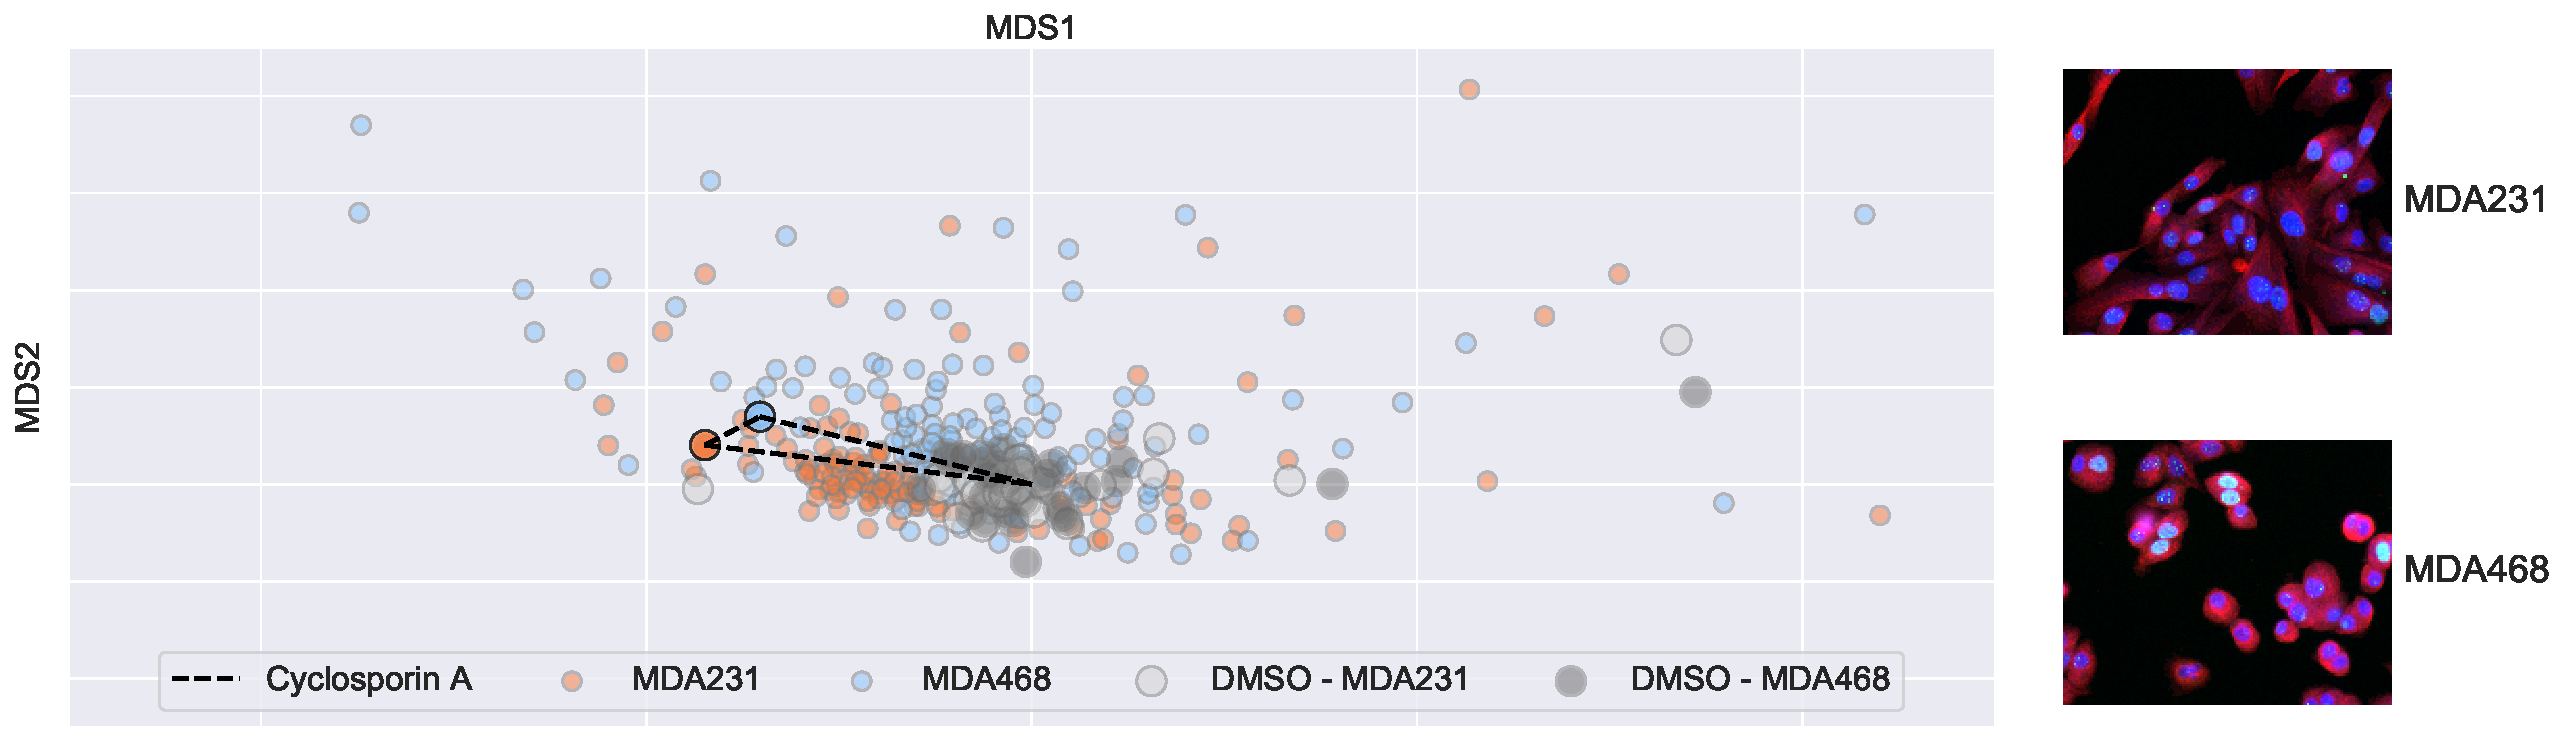
\includegraphics[width=\textwidth]{img/cyclosporin-A.pdf}
     }
     \hfill
     \subfloat[PKC-412 takes differential effects in the two cell lines.\label{subfig-2:dummy}]{%
       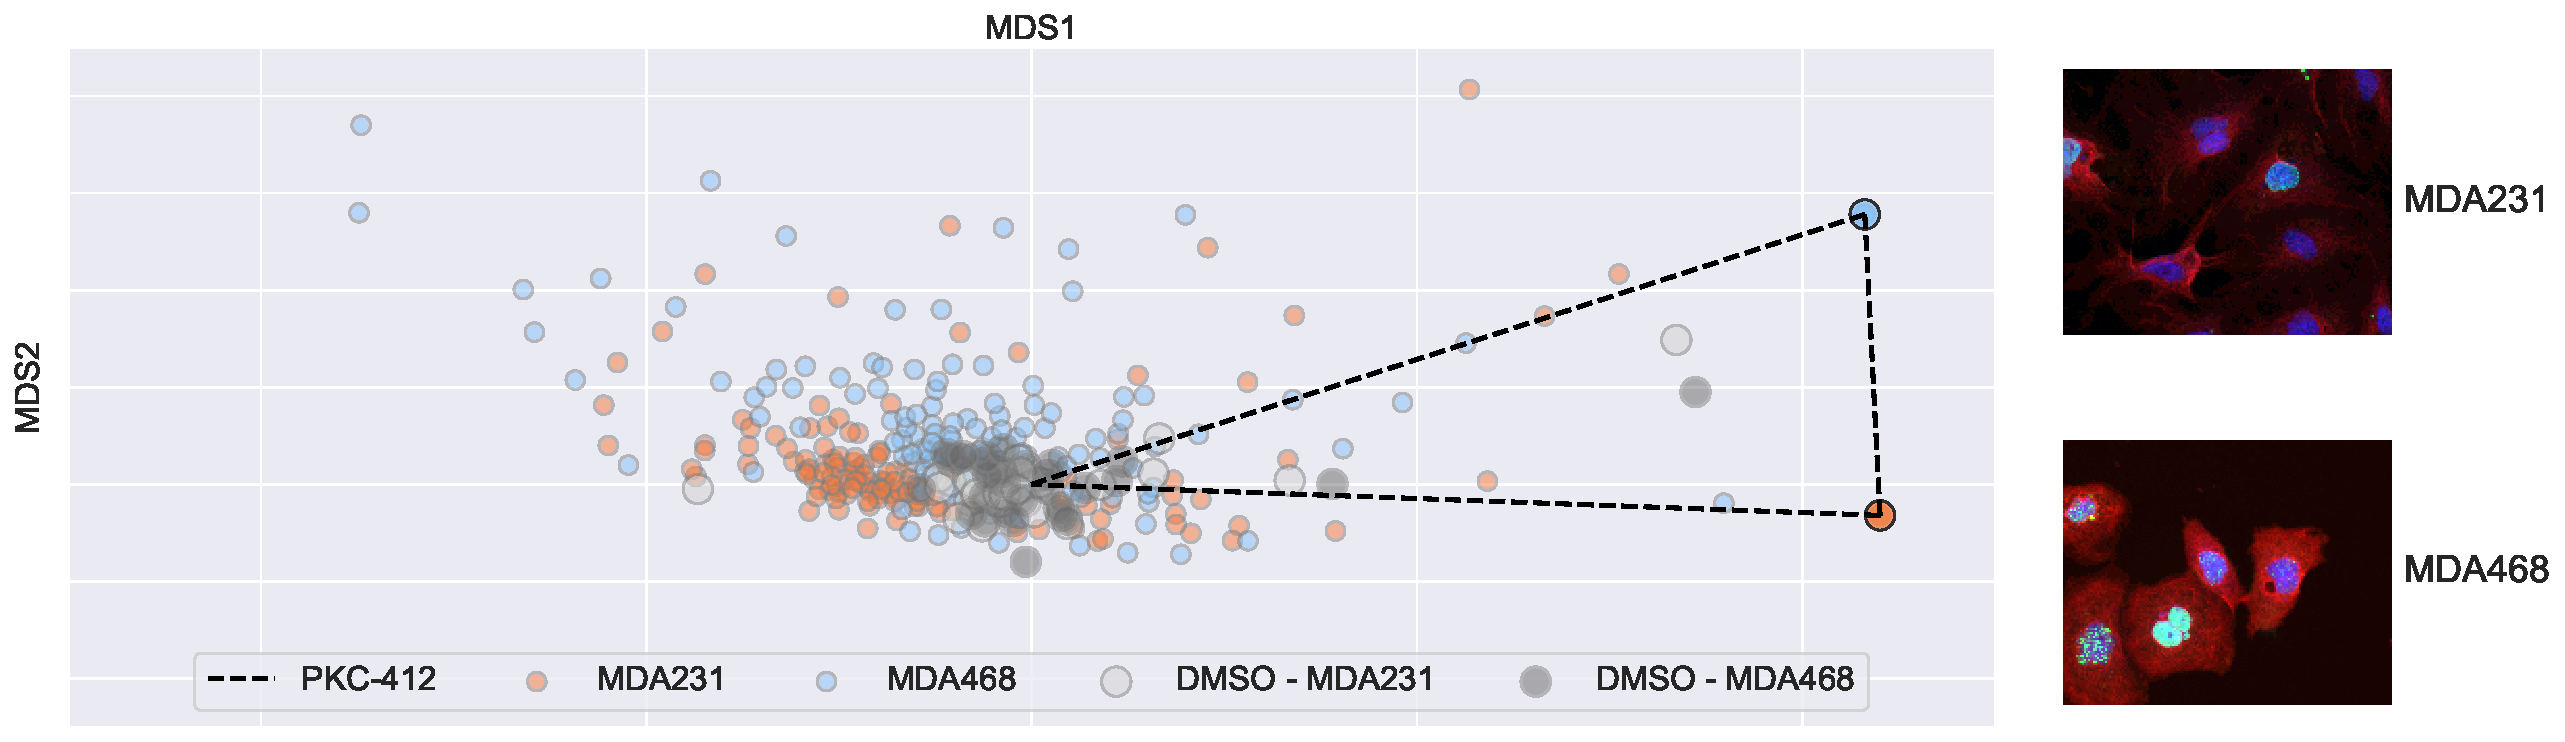
\includegraphics[width=\textwidth]{img/pkc-412.pdf}
     }
     \caption{MDS plots of each category of drug effect. The distances between the profiles are plotted as a line, as well as the respective distances to the centroid (origin).}
     \label{fig:dummy}
\end{figure}

\begin{figure}[h]%
    \centering
    \subfloat[$t = 42$]{{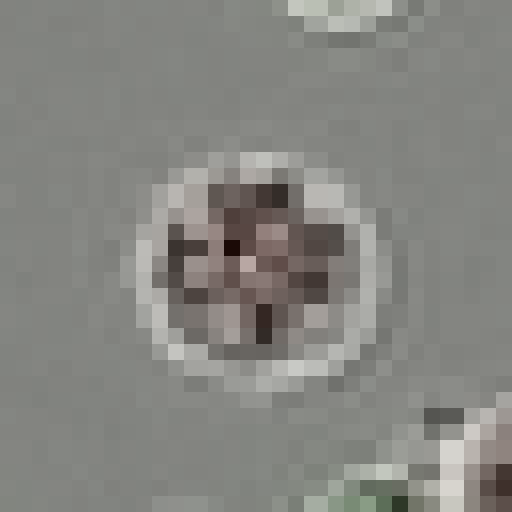
\includegraphics[width=0.25\textwidth]{img/r_t_cell_21.png}}}%
    \qquad
    \subfloat[$t = 44$]{{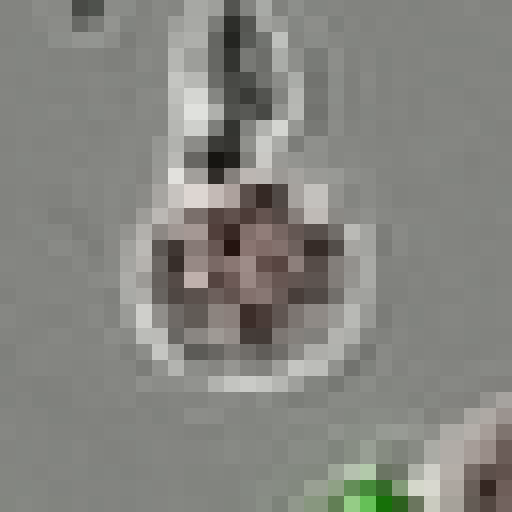
\includegraphics[width=0.25\textwidth]{img/r_t_cell_22.png}}}%
    \qquad
    \subfloat[$t = 92$]{{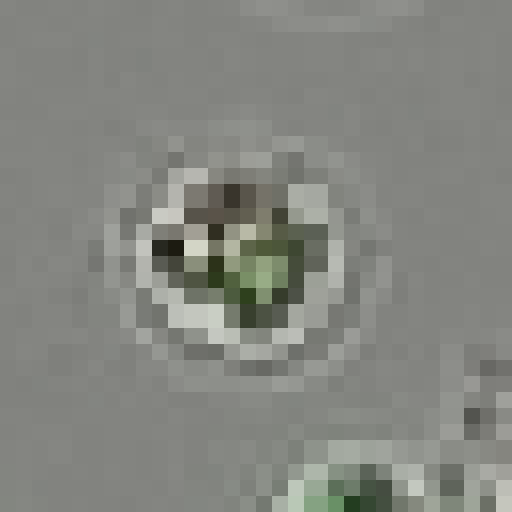
\includegraphics[width=0.25\textwidth]{img/r_t_cell_46.png}}}%
    \caption{A living Raji cell (a) is attacked by a CAR-T cell (b) and later dies (c).}%
    \label{fig:t_cell_latch}
\end{figure}

\begin{figure}[h]%
    \centering
    \subfloat[$t = 0$]{{
\includegraphics[width=0.25\textwidth]{img/r_dying_cell_0000.png}}}%
    \qquad
    \subfloat[$t = 2$]{{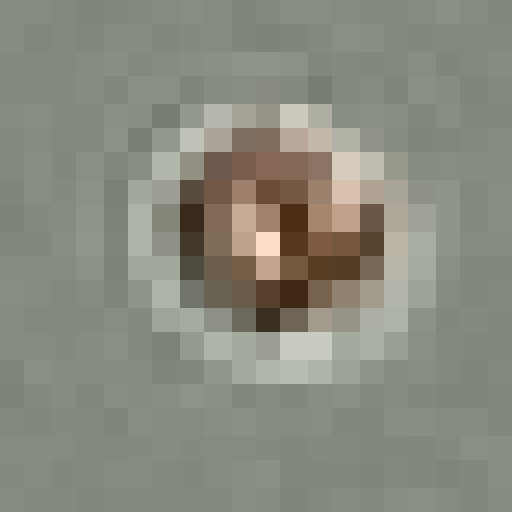
\includegraphics[width=0.25\textwidth]{img/r_dying_cell_0001.png}}}%
    \qquad
    \subfloat[$t = 4$]{{
\includegraphics[width=0.25\textwidth]{img/r_dying_cell_0002.png}}}%
    \qquad
    \subfloat[$t = 6$]{{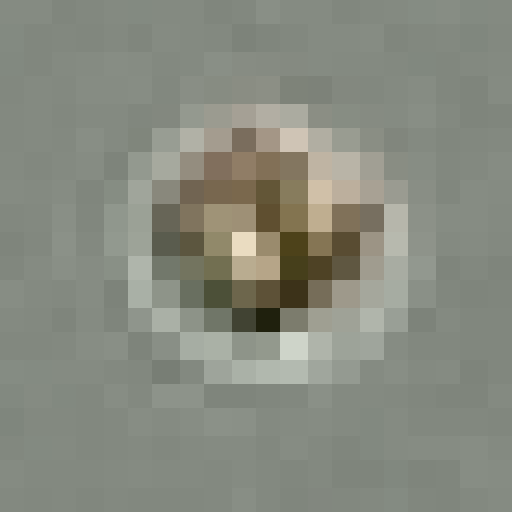
\includegraphics[width=0.25\textwidth]{img/r_dying_cell_0003.png}}}%
    \qquad
    \subfloat[$t = 8$]{{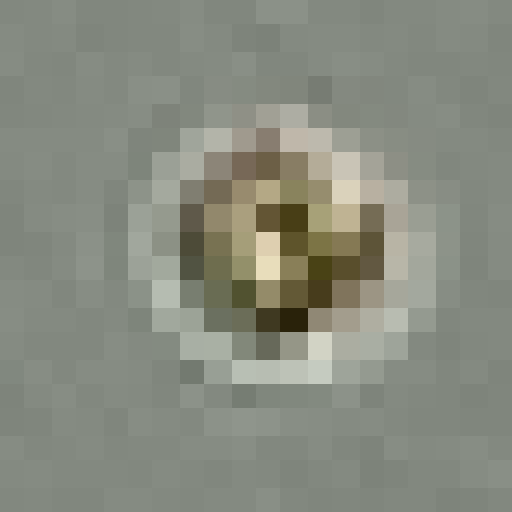
\includegraphics[width=0.25\textwidth]{img/r_dying_cell_0004.png}}}%
    \qquad
    \subfloat[$t = 10$]{{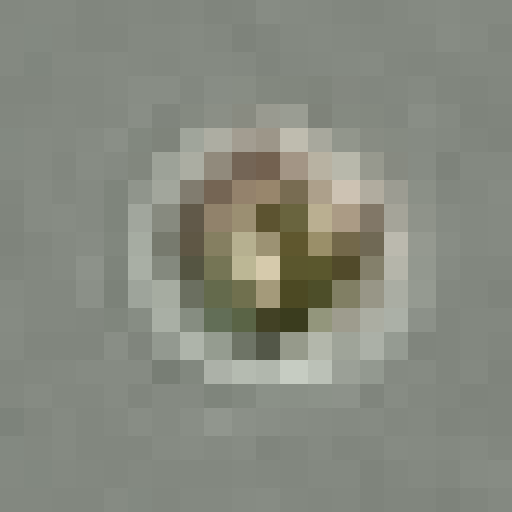
\includegraphics[width=0.25\textwidth]{img/r_dying_cell_0005.png}}}%
    \caption{Tracking the apoptosis of a Raji cell. Counterpart to Figure \ref{fig:dying_cell_series}.}
    \label{fig:dying_cell_frames}
\end{figure}

\begin{figure}[h]
\centering
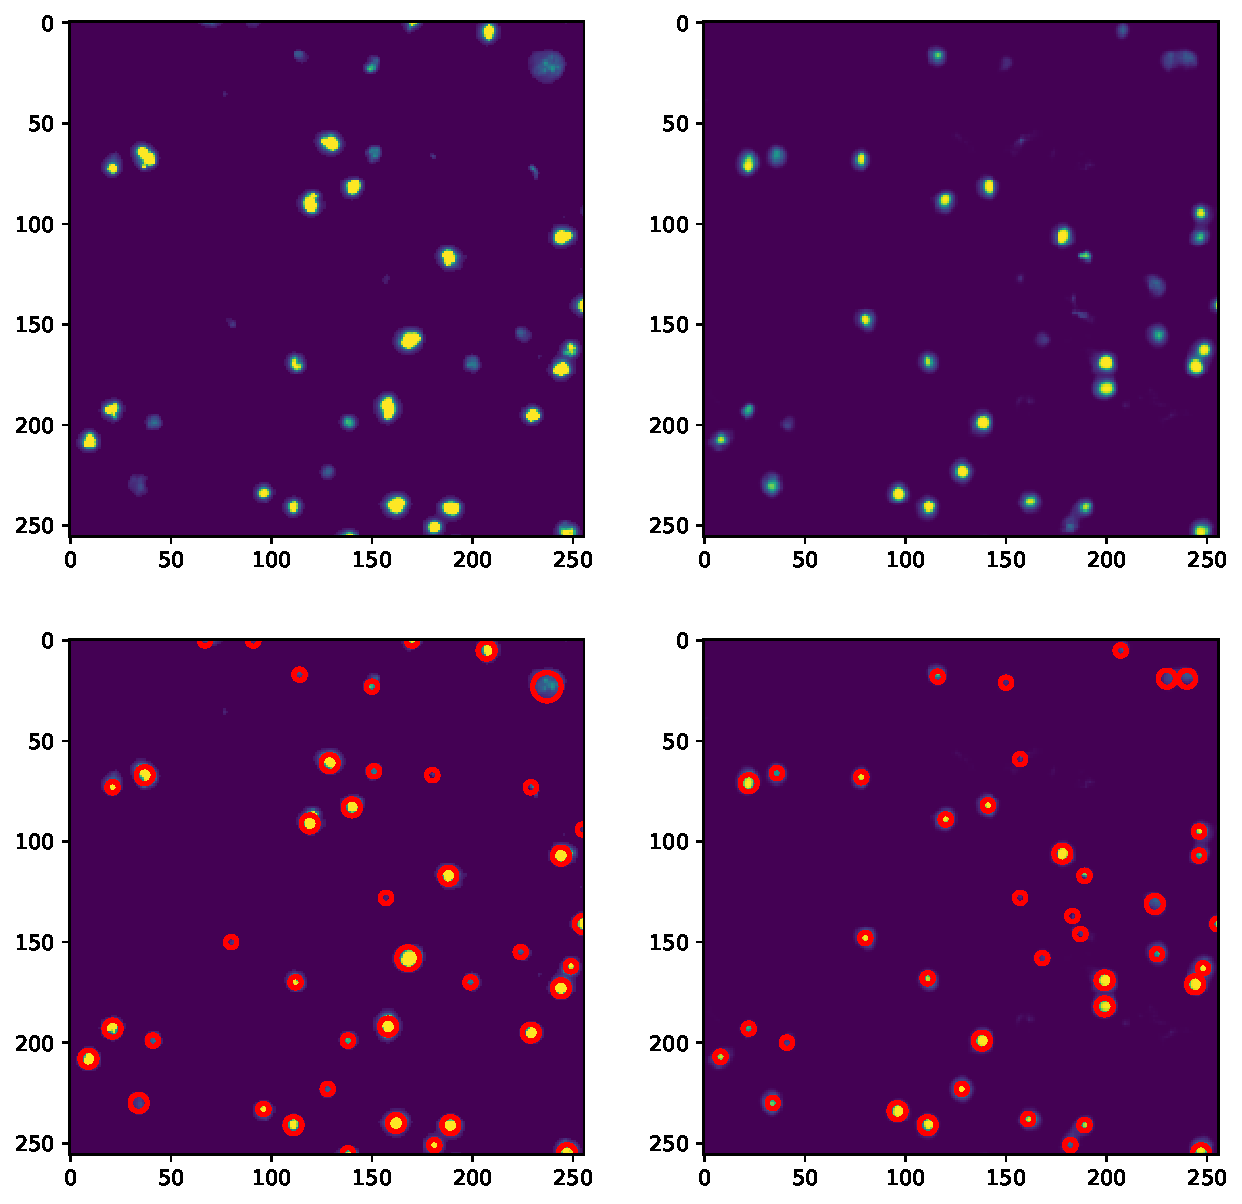
\includegraphics[width=0.85\textwidth]{img/blob_detection.pdf}
\caption{Blob detection results. Left column shows ground truth, right column shows \texttt{pix2pix} prediction. With respect to the ground truth: true positives: 31; false positives: 9; and false negatives: 11.}
\label{fig:blob_detection}
\end{figure}

\begin{figure}[h]%
    \centering
    \subfloat[mCherry]{{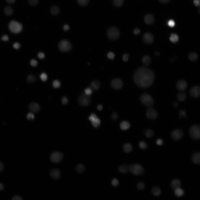
\includegraphics[width=0.25\textwidth]{img/pipeline_r.png} }}%
    \qquad
    \subfloat[GFP]{{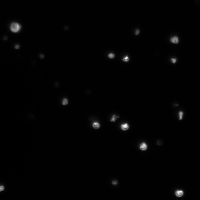
\includegraphics[width=0.25\textwidth]{img/pipeline_g} }}%
    \qquad
    \subfloat[Phase contrast]{{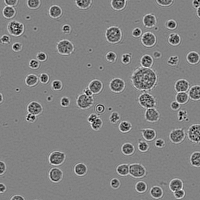
\includegraphics[width=0.25\textwidth]{img/pipeline_b.png} }}
    \qquad
    \subfloat[Background image]{{
\includegraphics[width=0.25\textwidth]{img/pipeline_segmentation_bg.png} }}%
    \qquad
    \subfloat[Segmentation]{{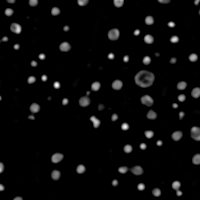
\includegraphics[width=0.25\textwidth]{img/pipeline_seg.png} }}%
    \qquad
    \subfloat[Fill holes]{{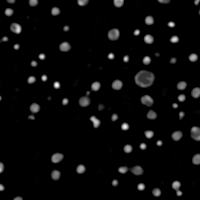
\includegraphics[width=0.25\textwidth]{img/pipeline_fill.png} }}
    \qquad
    \subfloat[Threshold]{{
\includegraphics[width=0.25\textwidth]{img/pipeline_mask.png} }}%
    \qquad
    \subfloat[Opening]{{
\includegraphics[width=0.25\textwidth]{img/pipeline_opened.png} }}%
    \qquad
    \subfloat[Labeling]{{
\includegraphics[width=0.25\textwidth]{img/pipeline_labels.png} }}
    \caption{An illustration of the automatic ground truth generation image processing pipeline. The first row are the image inputs.}%
    \label{fig:ground_truth_pipeline_example}%
\end{figure}
